\begin{figure}
	\centering
	\begin{subfigure}[b]{0.25\textwidth}
	    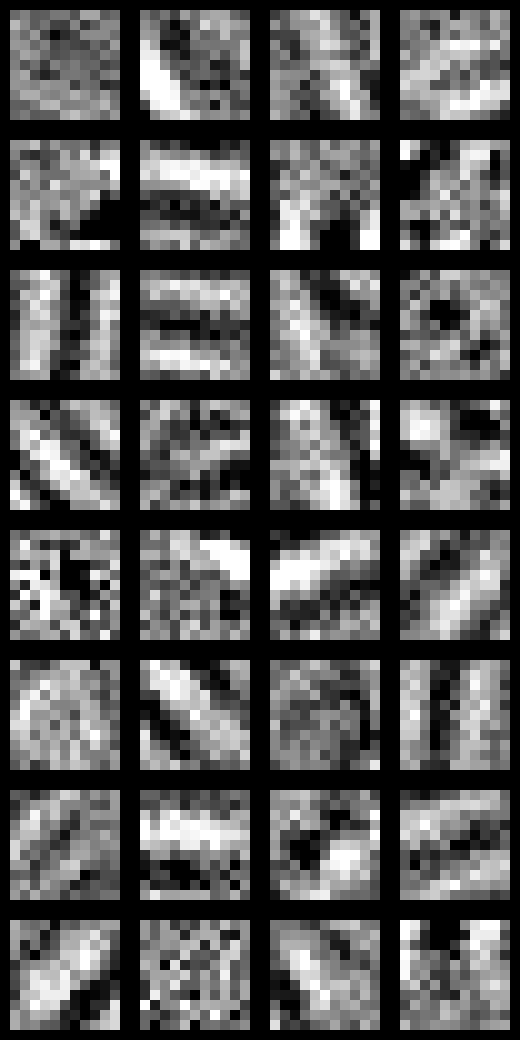
\epsfig{file=MSOEnet_filters_1.png, width = \textwidth}
		\vspace{-0.45cm}
		\caption{Frame 1}
	\end{subfigure}\hspace{5mm}%
	\begin{subfigure}[b]{0.25\textwidth}
	    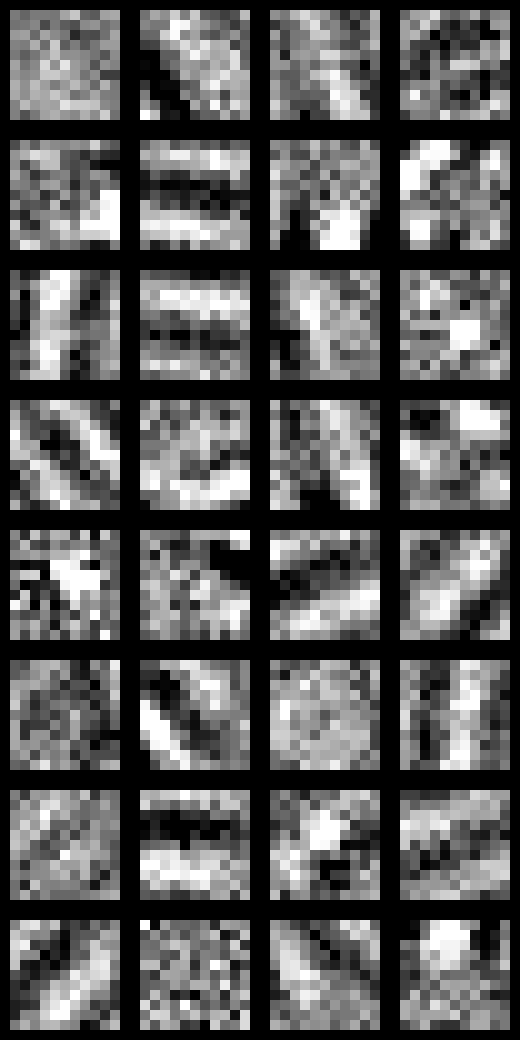
\epsfig{file=MSOEnet_filters_2.png, width = \textwidth}
		\vspace{-0.45cm}
		\caption{Frame 2}
	\end{subfigure}
	\caption[Learned spacetime-oriented filters]{32 learned spacetime-oriented filters of size $2 \times 11 \times 11$. (a) and (b) each depict a temporal slice of the learned filters, operating on the first and second frame of an input pair, respectively. Inspection of the learned filters reveals structures consistent with the handcrafted temporal derivative filters used in previous work \cite{derpanis2012spacetime} (\eg, row 3, col 1 captures rightward movement and row 8, col 1 captures down-right movement).}
	\label{fig:filters}
\end{figure}